\documentclass[12pt, a4paper]{article}

\usepackage{graphicx}
\usepackage[utf8]{inputenc}
\usepackage[italian]{babel}
\usepackage{hyperref}

%comandi personalizzati
\renewcommand{\labelitemi}{$\circ$}
\renewcommand{\labelitemii}{$\cdot$}
\renewcommand{\labelitemiii}{$\diamond$}
\renewcommand{\labelitemiv}{$\ast$}

%lettere accentate maiuscole
\newcommand*{\egrave}{\MakeUppercase{è} }

%settings dei links
\hypersetup{
	colorlinks=true,
	linkcolor=black,
	urlcolor=blue,
	pdftoolbar=true,
	pdfmenubar=true,
	pdftitle={English World},
	pdfauthor={Timoty Granziero, Elisa Giorio},
	pdfcreator={Timoty Granziero}	
}

\begin{document}

\frenchspacing
\begin{titlepage}
	\centering
	
\includegraphics[width=0.50\textwidth]{img/logo_unipd_color.png}\par\vspace{1cm} %logo
	
	{\LARGE\bfseries Progetto di Tecnologie Web \par}
	\vspace{1cm}
	
	{\Large\bfseries a.a. 2017/2018 \par}
	\vspace{1.5cm}
	
	{\Large Titolo della pagina web: \par}
	\vspace{0.5cm}
	
	{\LARGE\bfseries\itshape ENGLISH WORLD \par}
	
	\vfill 

	Autori: \par
	{\bfseries Elisa Giorio \par}
	{\bfseries Timoty Granziero \par}
	{\bfseries Edoardo Retis \par}
	
	\vfill

	Indirizzo del sito: \par
	\url{www.wikipedia.com}
	\vfill
	Autenticazione:\par
	email: \texttt{braian@libero.it}\par
	password: \texttt{brapol}
	\vfill
	
	% Bottom of the page
	{\large \today\par}
	
\end{titlepage}

%indice
\tableofcontents 
\pagebreak

\begin{abstract}
Con questo progetto ci poniamo di illustrare le attività proposte da una scuola privata di lingua inglese. La nostra piattaforma dovrà dare tutte le informazioni che uno studente, di qualsiasi età, cercherà in un sito; allo stesso tempo dovrà dare strumenti facili ai docenti per inserire le informazioni sulle lezioni, aule usate e sugli esami.\par
Ci saranno pagine dedicate ai corsi, per capire qual è il nostro livello di inglese; altre destinate alle lezioni e successivamente agli esami.
\end{abstract}

\section{Introduzione}

\subsection{Utenti destinatari}
Il sito internet sviluppato non vuole raggiungere una sola categoria di utenti, ma è destinato a chiunque cerchi una scuola di inglese.  Inoltre ogni utente potrà facilmente raccogliere le informazioni che cerca, sia che sia al primo accesso, sia un utente abituale del sito.\par
Il sito internet si propone come obbiettivo il raggiungimento di un utenza non solo giovane, bensì di qualsiasi età avvicinandola così alla tematica trattata.

\subsection{Lo scopo del sito web}
Il sito si propone di stabilire un canale di comunicazione sicuro e semplice tra la scuola e gli studenti che lo frequentano. A tal proposito abbiamo progettato il sito web concentrandoci sugli aspetti che potessero non solo dare all’utente la risposta che cerca, ma anche fornire un modo chiaro per farlo. Il sito web di fatto è semplice ed intuitivo, con una grafica non invasiva ma non per questo da ritenersi obsoleta.\par
\smallskip
All’interno del sito l’utente proverà una serie di corsi accompagnati da una breve descrizione. Una volta scelto il corso, ci saranno pagine dedicate allo svolgimento dei corsi e successivamente dell’esame.\par
\smallskip
%Oltre alla parte utente, il sito possiede anche una parte docente, dove proprio quest’ultimi possono prenotare aule per le lezioni o inserire gli orari e date degli esami.
Nei seguenti paragrafi verrà descritta la struttura del sito internet e suoi dettagli tecnici, elencando le tecnologie usate e le funzioni a disposizione. Verrà in particolar modo commentata l’accessibilità e l’usabilità del sito dimostrando quanto il progetto sia in linea con i moderni standard di progettazione.

\section{Gruppo di lavoro}
Al momento della conformazione del gruppo, ogni componente ha potuto decidere quale parte del progetto avrebbe preferito curare e realizzare. 
Il lavoro è stato così suddiviso:
\begin{itemize}
	\item Elisa Giorio: \texttt{HTML}, \texttt{CSS}, accessibilità e usabilità;
	\item Timoty Granziero: \texttt{PHP}, \texttt{MySQL}, \texttt{CSS};
	\item Edoardo Retis: ???
\end{itemize}

Per quanto riguarda la condivisione del materiale è stata usata la piattaforma di GitHub.

%\section{Gerarchia dei file}

%\subsection{Rappresentazione grafica}

%\subsection{Organizzazione interna}
 
\pagebreak %da vedere se ometterlo

\section{Progettazione concettuale}
Tutte le pagine principali seguono lo stesso schema ed è quello visto a lezione:
\begin{itemize}
	\item[\labelitemiii] \textit{Header}: dove sono presenti logo e titolo della pagina web;
	\item[\labelitemiii] \textit{Path}: indica dove ci troviamo all'interno del sito;
	\item[\labelitemiii] \textit{Menù}: menù a pannelli che indica quali pagine sono accessibili;
	\item[\labelitemiii] \textit{Corpo}: contiene i contenuti della pagina;
	\item[\labelitemiii] \textit{Footer}: utilizzato per inserire i loghi della validazione forniti da w3c, e il file .js per l’ultima modifica della pagina.
\end{itemize}

\begin{figure}[htb]
	\centering
	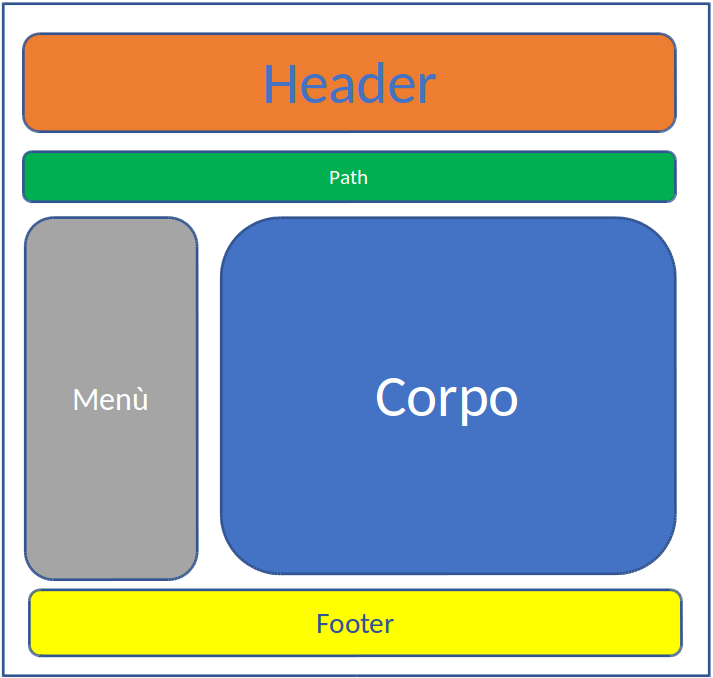
\includegraphics[height=9cm]{img/prog.png}
	\caption{Immagine che mostra il design del layout scelto.}	
\end{figure}

\section{Progettazione Logica}

\subsection{Parte utente}
Il sito dal punto di vista dell'utente è di tipo informativo. Egli può trovare nel sito
tutte le informazioni relativi ai corsi offerti e i contatti di tutti i docenti relativi
ad ogni corso. \egrave possibile inoltre consultare le prenotazioni delle aule per ogni
lezione ed esame.\par
Nella pagina \textit{contatti.php} è presente un frame di \emph{GMaps} che permette di 
raggiungere la posizione direttamente tramite Google Maps. \egrave presente un'alternativa 
testuale per chi non è in grado di visualizzare quel contenuto, a causa di vecchie tecnologie
o per problemi di disabilità.

\subsection{Parte docente}
Dal punto vi vista dell'utente loggato (un docente), alcune sezioni del sito
presentano alcune funzionalità aggiuntive: è possibile prenotare lezioni o esami negli 
appositi form. Sono stati inoltre implementati controlli sulla consistenza dei dati
processati via \texttt{PHP}, e per fare in modo che non sia possibile prenotare aule che sono già 
occupate a una determinata ora. \par

\subsection{Parte admin}
Una parte relativa all'\emph{admin} non è stata implementata all'interno del sito web 
perchè non ritenuta necessaria. L'admin infatti ha diretto accesso al codice sorgente
del sito e ai dati relativi dal database.

\section{Tecnologie}
Si è scelto di utilizzare le tecnologie principali necessarie per lo sviluppo web, senza
scomodare framework o altre librerie che per l'uso praticamente nullo che ne avremmo fatto
sarebbe stato un inutile incremento dei tempi di risposta della pagina web.

\subsection{Uso di Javascript}
Javascript viene usato principalmente per due script: l'ultima modifica (nel file \textit{ultima\_modifica.js}), e come codice embedded nel file \textit{corsi.php}.
\begin{itemize}
	\item \textbf{ultima\_modifica.js}: in questo script viene aggiornata la data di ultima modifica del file dove è chiamata la funzione \texttt{lastModify()}.
	\item \textbf{corsi.php}: in questa pagina, viene utilizzato uno script che visualizza la posizione della sede immaginaria (esattamente quella della 
	Torre Archimede di Padova) attraverso un frame di \textit{Google Maps}.
\end{itemize}

\subsection{Uso di PHP}
La parte relativa a PHP è piuttosto consistente. Nella cartella \textit{presets}, sono presenti 
alcuni script che, se inclusi tramite il comando \texttt{include()} di PHP, generano dimanicamente
una parte della pagina. \par
\smallskip
I file \textbf{header.php}, \textbf{footer.php} e \textbf{menu.php} generano rispettivamente la prima 
parte della pagina, il menù (assegnando dinamicamente valori di \texttt{tabindex} e la scheda attiva). \par
\smallskip
Nella cartella \textit{script}, sono presenti diversi script .php che eseguono controlli e comandi. Per interfacciarsi al database, si è scelto di utilizzare la libreria \texttt{mysqli}.\par
\smallskip
Un semplice script che genera codice relativo al login è \textbf{benvenuto.php}: chiede di accedere
in caso non ci sia un utente loggato, e da la possibilità di uscire in caso contrario. Lo script \textbf{logout.php} viene lanciato quando un utente loggato clicca su \texttt{Esci}. \par
Per verificare se il login avviene con successo e segnalare
gli eventuali errori, viene utilizzato lo script \textbf{validate\_form.php}. \par
Infine, \mbox{\textbf{validate\_prenotation.php}} e 
\mbox{\textbf{validate\_prenotation\_exams.php}} 
validano le prenotazioni relative rispettivamente alle lezioni e agli esami (per 
evitare sovrapposizioni), e in caso il controllo non riscontri problemi, le lezioni vengono inserite nel database.



\subsection{Uso di MySQL}
Come DBMS è stato scelto di utilizzare \texttt{MySQL}. Il database utilizzato è chiamato 
come il nome utente di laboratorio usato per la consegna: \textit{tgranzie}.\par 
I file utilizzati per popolare il database sono nella cartella \mbox{\textit{database}}: \mbox{\textit{table.sql}} per le tabelle, e \mbox{\textit{input.sql}} per il popolamento. 
Ecco l'elenco delle tabelle utilizzate con una breve descrizione:

\begin{itemize}
	\item \texttt{aule} contiene i dati relativi alle aule delle lezioni;
	\item \texttt{corsi} contiene l'elenco dei corsi disponibili nella scuola;
	\item in \texttt{docenti} ci sono i dati relativi ai docenti, comprese le 
	credenziali per effettuare il login;
	\item \texttt{lezioni} contiene le tuple relative alle prenotazioni delle 
	lezioni relative ai corsi.
	\item in \texttt{esami} è presente la lista degli esami relativi ai corsi;
\end{itemize}

\section{Validazione, Usabilità e Accessibilità}

\subsection{Validazione}
I controlli per la validazione sono stati fatti per ogni pagina del progetto tramite il
validatore W3C (\mbox{\url{https://validator.w3.org/}}). Tutte le pagine validano correttamente con \texttt{\mbox{XHTML Strict 1.0}}, eccezion fatta per la pagina contatti in cui il frame
di GMaps non valida. Viene per questo motivo nascosto in caso di vecchi browser.\par

\subsection{Usabilità}

\subsubsection{Resa dei browser}
L'usabilità delle pagine sui vari browser è stata testata tramite il sito web \mbox{\url{https://www.browserstack.com}}. I risultati ottenuti sono i seguenti:
\begin{itemize}
	\item[$-$] \textbf{Windows Chrome 63}: il sito è accessibile e valido;
	\item[$-$] \textbf{Firefox 40 per Windows 7}: il sito resta accessibile e valido.
\end{itemize}

I test effettuati su Internet Explorer sono stati fatti “a mano”. Questi sono i risultati:
\begin{itemize}
	\item[$-$] \textbf{IE 11}: il sito funziona correttamente, eccezione fatta per la 
	pagina \emph{contatti.php} in cui il frame di GMaps non funziona.
	\item[$-$] \textbf{IE 10} e \textbf{IE 8}: rilevato lo stesso problema di Internet Explorer 11. Per il resto, tutto viene visualizzato  correttamente. 
\end{itemize}

\subsubsection{Regola delle sei W}
Per fornire all’utente una navigazione gradevole nel sito, abbiamo cercato di rispettare 
la regola delle sei w:
\begin{itemize}
	\item \textbf{Who}: il sito in ogni pagina è molto riconoscibile, infatti grazie
	all’header l’utente capisce sempre in che pagina del sito si trova.
	\item \textbf{Where}: %l’utente può capire in ogni pagina dove si trova. Infatti il menù 
	%è sempre presente ed è sempre evidenziata la pagina attiva. Inoltre, path indica la
	%pagina attiva. In ogni pagina è sempre presente una piccola descrizione.
	l’utente può capire in ogni pagina dove si trova grazie al menù a lato; inoltre la pagina attiva è sia indicata nel path che evidenziata nel menù. \\
	In ogni pagina è sempre presente una piccola descrizione.
	\item \textbf{When}: tutte le pagine dinamiche vengono aggiornate costantemente. \\
	Nel footer è presente l’ultima modifica che rende facile anche all’utente capire se il
	 sito è attivo o meno;
	\item \textbf{Why}: le sezioni esami e lezioni, sono gli strumenti principali del sito.
	Qui l’utente può verificare gli orari delle lezioni. \\
	Anche per i docenti, queste due
	sezioni saranno le più usate. Infatti, come già detto, l'utente loggato ha la possibilità
	di prenotare lezioni e esami;
	\item \textbf{What}: premesso che la scuola d’inglese è una scuola puramente immaginaria 
	e non un ente commerciale, ci siamo impegnati a svilupparlo solo dal lato concettuale;
	\item \textbf{How}: il menù sempre presente, rende facile la navigazione all’interno
	della pagine. Non avendo sottomenù, la navigazione è ancora più semplice.
\end{itemize}

\subsection{Accessibilità}

\subsubsection{Separazione tra contenuto e presentazione}
\egrave stato scelto di seguire la good practice della totale separazione tra 
contenuto e presentazione. Infatti, la presentazione è interamente 
definita nei file \texttt{style.css} per il layout standard, \texttt{small.css}
per i dispositivi piccoli quali smartphone e palmari e \texttt{print.css} per la stampa.\par
Le porzioni di codice presenti in tutte le pagine, quali ad esempio l’\emph{header} e il \emph{menù}, sono presenti in script .php inclusi dinamicamente con l'istruzione \texttt{\mbox{include()}}, per evitare ridondanze di codice e promuovere la mantenibilità.

\subsubsection{Good practices}
Sono state seguite delle buone norme di coding per far sì che il sito sia accessibile a 
tutte le tipologie di utenti senza distinzione. \par
Come prima cosa, abbiamo utilizzato \texttt{span} con attributi \texttt{xml:lang} per definire correttamente termini che non sono nella lingua predefinita (nel nostro caso, abbiamo scelto di usare l'italiano come lingua principale nonostante sia un sito per 
lo studio della lingua inglese). \par
In secondo luogo, è presente un \texttt{link} non visibile che viene letto 
normalmente dagli screen reader, che permette agli utenti con deficit visivo di
saltare la navigazione (\texttt{nav}) per non doverla riascoltare ad ogni pagina.\par
\egrave stata posta particolare attenzione nell'uso dell'attributo \texttt{tabindex}: sono generati dalla variabile \texttt{\$tabindexCounter} di \texttt{PHP}. Ogni elemento che 
necessita di essere raggiunto dal \texttt{tab}, incrementa questa variabile e la stampa.

\subsubsection{Schema colori}
Per quanto riguarda l’uso dei colori sono state fatte delle prove di accessibilità sui sito
\mbox{\url{http://www.vischeck.com}}. I risultati, sono stati soddisfacenti, in quanto per problemi come Deuteranope, Protanope e Tritanope non sono stati rilevati cambiamenti drastici.\par
Questi sono i risultati ottenuti: \par

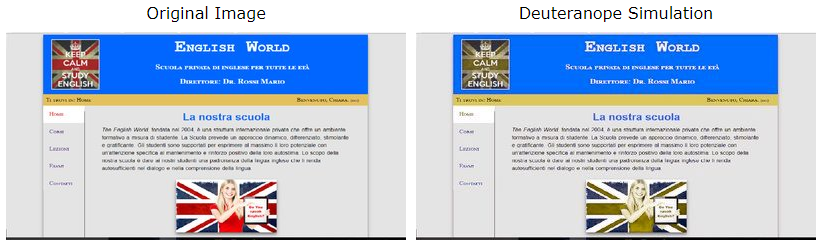
\includegraphics[height=4.5cm]{img/Deuteranope.PNG}\par
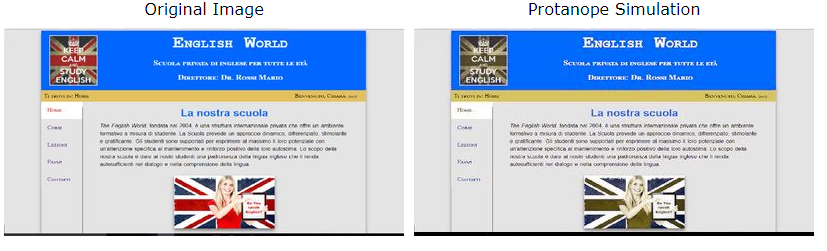
\includegraphics[height=4.5cm]{img/Protanope.PNG}\par
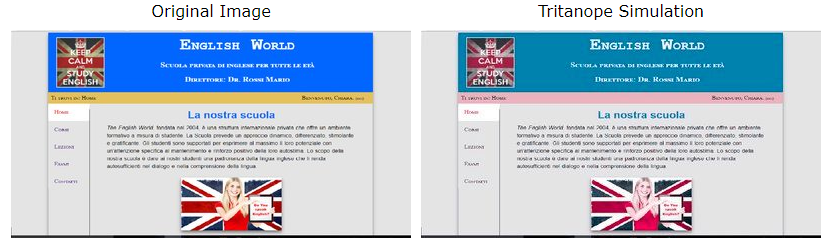
\includegraphics[height=4.5cm]{img/Tritanope.PNG}\par

I problemi sono stati rilevati in deuteranope e protanope per la visualizzazione del rosso,
ma questo non cambia la resa del sito. Mentre per la tritanope c’è un problema con la
visualizzazione del path, infatti il colore ocra non viene visto correttamente. Anche questo non crea nessun problema o cambio significativo nella resa del sito.\par

In conclusione, possiamo dire che le scelte di colori fatte possono essere adeguabili a tutti!

\section{Considerazioni finali}

\end{document}